\documentclass[oneside, a4paper]{memoir}

\usepackage[T1]{fontenc}
\usepackage{lmodern}
\usepackage{algpseudocode}
\usepackage{multirow}
\usepackage{longtable}
\usepackage[table]{xcolor}
\usepackage{tikz}
\usetikzlibrary{patterns}
\usepackage{contour}
\usepackage{microtype}
\usepackage[hidelinks]{hyperref}

\newcommand{\instruction}[6]{
\section{#1}
\section*{#2}
\subsection*{Usages}
#3
\subsection*{Description}
#4
\subsection*{Operation}
#5
\subsection*{Flags Affected}
\ifthenelse{\equal{#6}{}}{none}{#6}
\clearpage
}

\begin{document}
% Title
\title{SGPC Programmer's Manual}
\author{Steven Vroom}
\date{November 2016}
\maketitle
\cleardoublepage

\setlength\arrayrulewidth{1pt}
\rowcolors{2}{}{gray!15}

% Front Matter 
\frontmatter
\setcounter{tocdepth}{2}
\tableofcontents
\cleardoublepage
\listoffigures
\cleardoublepage
\listoftables
\cleardoublepage

\chapter{About This Manual}
\section{Related Documentation}
\section{Organization}
\section{Conventions}
\section{Acronyms and Abbreviations}

% Main Matter
\mainmatter
\chapter{Overview}
\section{SGPC Architecture Overview}
\section{Registers}
\subsection{User-accessible Registers}
\subsection{Internal Registers}
\section{Instruction Conventions}
\subsection{Instruction Layout}
\subsection{Addressing Modes}
\section{Instruction Set}
\section{Interrupt Model}
\section{Memory Management Model}

\chapter{Register Set}
This chapter describes the registers seperated in four groups based on accessability. however, the internal registers are omitted from this chapter since these are implementation specific.
\section{Foreground Registers}
The foreground registers are the registers all regular instructions can read from and write to. There are eight 8-bit and eight 16-bit foreground registers. These registers are preserved in interrupts.
\begin{table}[h]
\centering
\caption{List of Foreground Registers}
\label{tab:List of Foreground Registers}
\begin{tabular}{cclc}
\hiderowcolors
\textbf{ID}  & \textbf{Mnonic} & \textbf{Descriptive Name} & \textbf{Length in bits} \\ \hline
\showrowcolors
0x0 & al & The lower byte of ax  & 8  \\
0x1 & ah & The higher byte of ax & 8  \\
0x2 & bl & The lower byte of bx  & 8  \\
0x3 & bh & The higher byte of bx & 8  \\
0x4 & cl & The lower byte of cx  & 8  \\
0x5 & ch & The higher byte of cx & 8  \\
0x6 & dl & The lower byte of dx  & 8  \\
0x7 & dh & The higher byte of dx & 8  \\
0x8 & ax & The first GPR         & 16 \\
0x9 & bx & The second GPR        & 16 \\
0xA & cx & The third GPR         & 16 \\
0xB & dx & The fourth GPR        & 16 \\
0xC & ex & The fifth GPR         & 16 \\
0xD & tm & Temporary data        & 16 \\
0xE & sp & Stack pointer         & 16 \\
0xF & pc & Program counter       & 16 \\
\end{tabular}
\end{table}
\subsection{General-Purpose Registers (GPRs)}
These registers are meant for computing storage. The first four 16-bit registers are all splitted into two 8-bit registers. So software can directly access the upper and lower byte of these 16-bit registers.
\subsection{Temporary Data Register}
This registers is meant to facilitate call procedures. So it won't be preserved in a function call. However this nothing more than a suggestion to the user, software can use this register as a regular GPR.
\subsection{Stack Pointer Register (SP)}
This register is meant to keep track of the end of the stack. However this nothing more than a suggestion to the user, software can use this register as a regular GPR.
\subsection{Program Counter Register (PC)}
This register holds the address of the next instruction to run. Writing to this registers means jumping to other code.
\section{Background Registers}
Background registers can only accessed with the instructions BSTR and BLD.
\begin{table}[h]
\centering
\caption{List of Background Registers}
\label{tab:List of Background Registers}
\begin{tabular}{cclc}
\hiderowcolors
\textbf{ID}  & \textbf{Mnonic} & \textbf{Descriptive Name} & \textbf{Length in bits} \\ \hline
\showrowcolors
0x0 & n/a & Reserved                  & 8  \\
0x1 & n/a & Reserved                  & 8  \\
0x2 & n/a & Reserved                  & 8  \\
0x3 & n/a & Reserved                  & 8  \\
0x4 & n/a & Reserved                  & 8  \\
0x5 & n/a & Reserved                  & 8  \\
0x6 & n/a & Reserved                  & 8  \\
0x7 & n/a & Reserved                  & 8  \\
0x8 & bpc & Program counter backup    & 16 \\
0x9 & bsf & Segments and flags backup & 16 \\
0xA & ipc & Interrupt program counter & 16 \\
0xB & is  & Interrupt segments        & 16 \\
0xC & n/a & Reserved                  & 16 \\
0xD & n/a & Reserved                  & 16 \\
0xE & n/a & Reserved                  & 16 \\
0xF & n/a & Reserved                  & 16 \\
\end{tabular}
\end{table}
\subsection{Backup Registers}
The backup registers are used to backup the state of the CPU (see \autoref{sec:State Preservation}). The foreground registers, segment registers and flags register all have their own backup register. However, most backup register aren't background registers. Only the segment registers, program counter register and flags register have directly accessable backup registers. Note that both segment registers and the flag register share one 16-bit backup register.
\begin{description}
\item[CS]: The code segment, This holds the index of the segment that is used to fetch instructions from the memory (see \autoref{}).
\item[DS]: The data segment, This holds the index of the segment that is used to read data from and write data to the memory (see \autoref{}).
\item[Z, S, P, O, C and I]: The flags, these hold data about the state of the processor or control how the processor behaves (see \autoref{sub:Flags Register})
\end{description}
\begin{figure}[h!]
\begin{center}
\caption{Segments and Flags Backup Register's Layout}
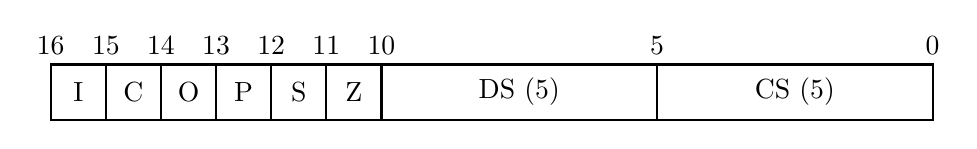
\begin{tikzpicture}[scale=.7]
\draw [thick] (0,0) rectangle (1,-1) node[pos=.5] {I};
\node[above] at (0,0) {16};
\node[above] at (1,0) {15};
\draw [thick] (1,0) rectangle (2,-1) node[pos=.5] {C};
\node[above] at (2,0) {14};
\draw [thick] (2,0) rectangle (3,-1) node[pos=.5] {O};
\node[above] at (3,0) {13};
\draw [thick] (3,0) rectangle (4,-1) node[pos=.5] {P};
\node[above] at (4,0) {12};
\draw [thick] (4,0) rectangle (5,-1) node[pos=.5] {S};
\node[above] at (5,0) {11};
\draw [thick] (5,0) rectangle (6,-1) node[pos=.5] {Z};
\node[above] at (6,0) {10};
\draw [thick] (6,0) rectangle (11,-1) node[pos=.5] {DS (5)};
\node[above] at (11,0) {5};
\draw [thick] (11,0) rectangle (16,-1) node[pos=.5] {CS (5)};
\node[above] at (16,0) {0};
\end{tikzpicture}
\end{center}
\end{figure}
\subsection{Interrupt Registers}
The Interrupt registers hold the new state the CPU should jump to when an interrupt is triggered (see \autoref{ch:Interrupts}). Only the segement registers and the program counter have an interrupt register.
\begin{description}
\item[CS]: The code segment, This holds the index of the segment that is used to fetch instructions from the memory (see \autoref{}).
\item[DS]: The data segment, This holds the index of the segment that is used to read data from and write data to the memory (see \autoref{}).
\end{description}
\begin{figure}[h!]
\begin{center}
\caption{Segments Interrupt Register's Layout}
\contourlength{1pt}
\contournumber{20}
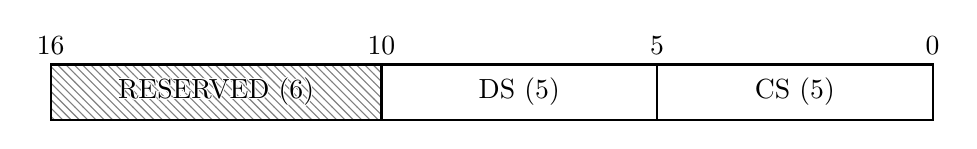
\begin{tikzpicture}[scale=.7]
\draw[thick, pattern=north west lines, pattern color=gray] (0,0) rectangle (6,-1) node[pos=.5] {\contour{white}{RESERVED (6)}};
\node[above] at (0,0) {16};
\node[above] at (6,0) {10};
\draw[thick] (6,0) rectangle (11,-1) node[pos=.5] {DS (5)};
\node[above] at (11,0) {5};
\draw[thick] (11,0) rectangle (16,-1) node[pos=.5] {CS (5)};
\node[above] at (16,0) {0};
\end{tikzpicture}
\end{center}
\end{figure}
\section{Indirect Registers}
Indirect registers are registers that software can't directly read nor write to with any instruction. All the backup registers that aren't background registers fall under this catogory. All the indirect registers can only be written to and read from via the state preservation system (see \autoref{sec:State Preservation}).
\subsection{Flags Register}
\label{sub:Flags Register}
The flags register holds multiple flags (see \autoref{tab:List of Flags}). There are two types of flags: status flags and control flags. Status flags give software extra information about the last computation made, while control flags control how the cpu behaves. There is only one control flag in the [insert name here] processor, the interrupts enabled flag. If this flag is set to zero interrupt requests will be ignored (see \autoref{sec:Interrupt Enabling/Disabling}).
\begin{description}
\item[Zero flag]: If the result of the last computation is equal to zero this flag will be set, otherwise it will be cleared.
\item[Sign flag]: If the most significant  bit of the result of the last computation is set this flag will be set, otherwise it will be cleared.
\item[Parity flag]: If the least significant  bit of the result of the last computation is clear this flag will be set, otherwise it will be cleared.
\item[Overflow flag]: If the signed two's-complement result of the last computation is too large to fit in operand A (see \autoref{sec:Operand Conventions}) this flag will be set, otherwise it will be cleared. (Not all computational instructions change this flag)
\item[Carry flag]: If the unsigned result of the last computation is too large to fit in operand A (see \autoref{sec:Operand Conventions}) this flag will be set, otherwise it will be cleared. (Not all computational instructions change this flag)
\end{description}
\begin{table}[h]
\centering
\caption{List of Flags}
\label{tab:List of Flags}
\begin{tabular}{cllc}
\hiderowcolors
\textbf{Mnonic} & \textbf{Descriptive Name} & \textbf{Type of flag} & \textbf{Length in bits} \\ \hline
\showrowcolors
Z & Zero flag               & Status flag  & 1 \\
S & Sign flag               & Status flag  & 1 \\
P & Parity flag             & Status flag  & 1 \\
O & Overflow flag           & Status flag  & 1 \\
C & Carry flag              & Status flag  & 1 \\
I & Interrupts enabled flag & Control flag & 1 \\
\end{tabular}
\end{table}
\subsection{Segment Registers}
The segment registers (see \autoref{tab:List of Segment Registers}) hold the index of the segments currently used (see \autoref{ch:Memory Management}).
\begin{table}[h]
\centering
\caption{List of Segment Registers}
\label{tab:List of Segment Registers}
\begin{tabular}{clc}
\hiderowcolors
\textbf{Mnonic} & \textbf{Descriptive Name} & \textbf{Length in bits} \\ \hline
\showrowcolors
CS & Code segment index & 5 \\
DS & Data segment index & 5 \\
\end{tabular}
\end{table}
\section{Output Registers}
The output registers (see \autoref{tab:List of Output Registers}) hold information that is sent to the pheripherals (see \autoref{ch:I/O Conventions})
\begin{table}[h!]
\centering
\caption{List of Output Registers}
\label{tab:List of Output Registers}
\begin{tabular}{clc}
\hiderowcolors
\textbf{Mnonic} & \textbf{Descriptive Name} & \textbf{Length in bits} \\ \hline
\showrowcolors
AO & The first output register   & 16 \\
BO & The second output register  & 16 \\
CO & The third output register   & 16 \\
DO & The fourth output register  & 16 \\
EO & The fifth output register   & 16 \\
FO & The sixth output register   & 16 \\
GO & The seventh output register & 16 \\
HO & The eigth output register   & 16 \\
\end{tabular}
\end{table}

\chapter{Operand Conventions}
\label{ch:Operand Conventions}
This chapter describes the possible operands and how to use them. The operands are seperated into normal operands and special operands. 
\section{Operands in Instructions}
All instructions have two operands, however, some instructions don't use them or only use one. The two operands have a set role. Operand A (the first operand after the instruction) is the output and the secondary input. Operand B (the second operand after the instruction) is the primary input. In other words the processor generally follows this behaviour: read B, optionaly read A, calculate and finally write to A.
\section{Normal Operands}
Normal operands simply access the foreground registers. This type of operands is ensured to take the least amount of read and write time, so it is advised to use this operand type for computations.
\subsection{Exception: ISTR \& ILD}
The ISTR and ILD alter the behaviour of the normal A and B operands respectively. Instead of the foreground registers the operands access the background registers. There are only four background registers. If ISTR or ILD try to access any of the reserved background register the behaviour of that instruction is undefined.
\section{Special Operands}
Special operands make use of the immidiate of an instruction. If both operands of an instruction are special operands then they share the \underline{same} immidiate. The A and B operand have different special operands.
\subsection{Special Operand A}
Special operand A is used to access the memory. The operands adds a register to the immidiate and uses the answer of that calculation as memory address. It's also possible to use the immidiate as address directly without the addition. It's possible to read and write both 8-bits and 16-bit.
\subsection{Special Operand B}
Special operand B can both be used access the memory or directly. The operands either adds a register to the immidiate and uses the answer of that calculation as memory address, or just uses the answer of the calculation directly as the value of the operand. It's also possible to use the immidiate as address or value directly without the addition.
\section{List of Operands}

\begin{center}
\begin{longtable}{cclc}
\caption{List of Operands} 
\label{tab:List of Operands} \hline
\endfirsthead
\hiderowcolors
\textbf{ID}  & \textbf{Mnonic} & \textbf{Description} & \textbf{\vtop{\hbox{\strut Length}\hbox{\strut in bits}}} \\ \hline
\showrowcolors 
\endhead
\hiderowcolors
\multicolumn{4}{c}{\textbf{Normal Operands}} \\ \hline
\showrowcolors
0x00 & al  & The lower byte of ax      & 8  \\
0x01 & ah  & The higher byte of ax     & 8  \\
0x02 & bl  & The lower byte of bx      & 8  \\
0x03 & bh  & The higher byte of bx     & 8  \\
0x04 & cl  & The lower byte of cx      & 8  \\
0x05 & ch  & The higher byte of cx     & 8  \\
0x06 & dl  & The lower byte of dx      & 8  \\
0x07 & dh  & The higher byte of dx     & 8  \\
0x08 & ax  & The first GPR             & 16 \\
0x09 & bx  & The second GPR            & 16 \\
0x0A & cx  & The third GPR             & 16 \\
0x0B & dx  & The fourth GPR            & 16 \\
0x0C & ex  & The fifth GPR             & 16 \\
0x0D & tm  & Temporary data            & 16 \\
0x0E & sp  & Stack pointer             & 16 \\
0x0F & pc  & Program counter           & 16 \\ \hline
\hiderowcolors
\multicolumn{4}{c}{\textbf{Exceptions: Operand A of ISTR \& Operand B of ILD}} \\ \hline
\showrowcolors
0x00 & n/a & Reserved                  & 8  \\
0x01 & n/a & Reserved                  & 8  \\
0x02 & n/a & Reserved                  & 8  \\
0x03 & n/a & Reserved                  & 8  \\
0x04 & n/a & Reserved                  & 8  \\
0x05 & n/a & Reserved                  & 8  \\
0x06 & n/a & Reserved                  & 8  \\
0x07 & n/a & Reserved                  & 8  \\
0x08 & bpc & Program counter backup    & 16 \\
0x09 & bsf & Segments and flags backup & 16 \\
0x0A & ipc & Interrupt program counter & 16 \\
0x0B & is  & Interrupt segments        & 16 \\
0x0C & n/a & Reserved                  & 16 \\
0x0D & n/a & Reserved                  & 16 \\
0x0E & n/a & Reserved                  & 16 \\
0x0F & n/a & Reserved                  & 16 \\ \hline
\hiderowcolors
\multicolumn{4}{c}{\textbf{Exception: Operand A of OUT}} \\ \hline
\showrowcolors
0x00 & AO & The first output register   & 16 \\
0x01 & BO & The second output register  & 16 \\
0x02 & CO & The third output register   & 16 \\
0x03 & DO & The fourth output register  & 16 \\
0x04 & EO & The fifth output register   & 16 \\
0x05 & FO & The sixth output register   & 16 \\
0x06 & GO & The seventh output register & 16 \\
0x07 & HO & The eigth output register   & 16 \\
0x08 & n/a & Reserved                  & 16 \\
0x09 & n/a & Reserved                  & 16 \\
0x0A & n/a & Reserved                  & 16 \\
0x0B & n/a & Reserved                  & 16 \\
0x0C & n/a & Reserved                  & 16 \\
0x0D & n/a & Reserved                  & 16 \\
0x0E & n/a & Reserved                  & 16 \\
0x0F & n/a & Reserved                  & 16 \\ \hline
\hiderowcolors
\multicolumn{4}{c}{\textbf{Special Operands A}} \\ \hline
\showrowcolors
0x10 & [ax+\#]  & The byte at: ax plus the immidiate & 8 \\
0x11 & [bx+\#]  & The byte at: bx plus the immidiate & 8 \\
0x12 & [cx+\#]  & The byte at: cx plus the immidiate & 8 \\
0x13 & [dx+\#]  & The byte at: dx plus the immidiate & 8 \\
0x14 & [fx+\#]  & The byte at: fx plus the immidiate & 8 \\
0x15 & [pc+\#]  & The byte at: pc plus the immidiate & 8 \\
0x16 & [sp+\#]  & The byte at: sp plus the immidiate & 8 \\
0x17 & [\#]     & The byte at: the immidiate & 8 \\
0x18 & @[ax+\#] & The word at: ax plus the immidiate & 16 \\
0x19 & @[bx+\#] & The word at: bx plus the immidiate & 16 \\
0x1A & @[cx+\#] & The word at: cx plus the immidiate & 16 \\
0x1B & @[dx+\#] & The word at: dx plus the immidiate & 16 \\
0x1C & @[fx+\#] & The word at: fx plus the immidiate & 16 \\
0x1D & @[pc+\#] & The word at: pc plus the immidiate & 16 \\
0x1E & @[sp+\#] & The word at: sp plus the immidiate & 16 \\
0x1F & @[\#]    & The word at: the immidiate         & 16 \\ \hline
\hiderowcolors
\multicolumn{4}{c}{\textbf{Special Operands B}} \\ \hline
\showrowcolors
0x10 & [ax+\#]  & Memory from: ax plus the immidiate & same as A \\
0x11 & [bx+\#]  & Memory from: bx plus the immidiate & same as A \\
0x12 & [cx+\#]  & Memory from: cx plus the immidiate & same as A \\
0x13 & [dx+\#]  & Memory from: dx plus the immidiate & same as A \\
0x14 & [fx+\#]  & Memory from: fx plus the immidiate & same as A \\
0x15 & [pc+\#]  & Memory from: pc plus the immidiate & same as A \\
0x16 & [sp+\#]  & Memory from: sp plus the immidiate & same as A \\
0x17 & [\#]     & Memory from: the immidiate         & same as A \\
0x18 & ax+\# & ax plus the immidiate & 16 \\
0x19 & bx+\# & bx plus the immidiate & 16 \\
0x1A & cx+\# & cx plus the immidiate & 16 \\
0x1B & dx+\# & dx plus the immidiate & 16 \\
0x1C & fx+\# & fx plus the immidiate & 16 \\
0x1D & pc+\# & pc plus the immidiate & 16 \\
0x1E & sp+\# & sp plus the immidiate & 16 \\
0x1F & \#    & the immidiate         & 16 \\
\end{longtable}
\end{center}


\chapter{Addressing}
\label{ch:Addressing}
\section{Bit and Byte Ordering}
\section{Aligned and Misaligned Memory Access}


\chapter{Instruction Set Summary}
\label{ch:Instruction Set Summary}
This chapter gives a summary on the instruction set of the ABCD processor. It will describe the types of instructions and the binary layout of the instructions.
\section{Instruction Types}
The instructions can be seperated in five types. Two of these types are not meant to be used. 
\subsection{Move Instructions}
The move instructions copy data from it's source operand to it's target operand. The simpelest move instruction is MOV and does just that. The rest of the move instructions are conditional move instructions, these only copy data when certain conditions are met. These conditions all have to do with previous calculations and use the flags register.
\begin{description}
\item[MOVZ]: Move if the zero flag is set.
\item[MOVNZ]: Move if the zero flag is clear.
\item[MOVS]: Move if the sign flag is set.
\item[MOVNS]: Move if the sign flag is clear.
\item[MOVP]: Move if the parity flag is set.
\item[MOVNP]: Move if the parity flag is clear.
\item[MOVO]: Move if the overflow flag is set.
\item[MOVNO]: Move if the overflow flag is clear.
\item[MOVC]: Move if the carry flag is set.
\item[MOVNC]: Move if the carry flag is clear.
\item[MOV=]: Move if the previous comparison was equal.
\item[MOV!=]: Move if the previous comparison was unequal.
\item[MOVU<]: Move if the previous comparison of unsigned integers was smaller.
\item[MOVU<=]: Move if the previous comparison of unsigned integers was smaller or equal.
\item[MOVU>=]: Move if the previous comparison of unsigned integers was greater or equal.
\item[MOVU>]: Move if the previous comparison of unsigned integers was greater.
\item[MOVS<]: Move if the previous comparison of signed integers was smaller.
\item[MOVS<=]: Move if the previous comparison of signed integers was smaller or equal.
\item[MOVS>=]: Move if the previous comparison of signed integers was greater or equal.
\item[MOVS>]: Move if the previous comparison of signed integers was greater.
\end{description}
\subsection{Addition and Subtraction Instructions}
There preform binary addition and subtraction for both signed and unsigned integers. In all the addition instructions you can two's compliment negate one of the operands. A substraction instruction is an addition instruction with the B operand negated. There are three groups of addition/subtraction instructions:
\begin{description}
\item[ADD / SUB]: Add/subtract the two operands.
\item[ADD1 / SUB1]: Add/subtract the two operands and add/subtract 1.
\item[ADDC / SUBB]: Add/subtract the two operands and, if the carry flag is set, add/subtract 1.
\end{description}
\subsection{Logical Instructions}
The logical instructions preform simple bitwise logical functions. In all logical Instructions you can one's compliment negate (NOT) one or both of the operands.
\begin{description}
\item[OR]: Perform bitwise logical OR.
\item[AND]: Perform bitwise logical AND.
\item[XOR]: Perform bitwise logical XOR.
\end{description}
\subsection{Bit Shifting Instructions}
The bit shifting instructions shift or rotate the bits of its operand by one bit.
\begin{description}
\item[SHL]: Shifts all bits one bit left and clears the new least significant bit.
\item[SHR]: Shifts all bits one bit right and clears the new most significant bit.
\item[SHL1]: Shifts all bits one bit left and sets the new least significant bit.
\item[SHR1]: Shifts all bits one bit right and sets the new most significant bit.
\item[ROL]: Shifts all bits one bit left and writes the old most significant bit to the new least significant bit.
\item[ROR]: Shifts all bits one bit right and writes the old least significant bit to the new most significant bit
\item[RCL]: Shifts all bits one bit left and clears new the least significant bit.
\item[RCR]: Shifts all bits one bit right and clears new the most significant bit.
\end{description}
\subsection{Control Instructions}
Control Instruction change specific parts of the processor state. Unlike the move and computational instructions these instructions don't necessarily read from operand B and write/read from A .
\begin{description}
\item[WRI]: Sets or clears the I flag.
\item[ISTR]: Writes to an background register.
\item[ILD]: Writes from an background register.
\item[OUT]: Writes to an output register.
\item[IN]: Request input from a pheriperal.
\item[BACK]: Backup the most registers.
\item[FRET]: Fully restore the last backup and marks and marks any running interrupt done.
\item[PRET]: Restore the program counter and the stack pointer from the last backup and marks any running interrupt done.
\item[FJMP]: Restore the program counter and the stack pointer from the last backup.
\item[HLT]: Halts the processor untill a interrupt is triggered.
\item[NOP]: Does nothing but delay the processor a bit.
\end{description}
\subsection{Reserved Instructions}
Reserved instructions are instructions with undefined behaviour, meaning they can do anything to the state of the CPU or the RAM. Reserved instructions should never be used in code. However, reserved instructions will never message pheripers, so it's impossible to change non-volatile memory or damage any components. Thus any problems that reserved instructions invoke directly will not persist after restarting the system. 
\subsection{Artifact Instructions}
Artifact instructions are instructions with defined behaviour, but aren't considererd a permanent part of the ABCD processor family. These instructions tend to only exist because it would take more parts to remove them than it takes to leave them in.

\section{Instruction Format}
All instructions follow one single format. The format has four parts:
\begin{description}
\item[OP]: The opcode, this describes what operation will be excecuted by this instruction (see \autoref{app:Instruction Set Listings}).
\item[A]: Operand A, This describes what the instruction will use as output and secondary input (see \autoref{tab:List of Operands}).
\item[B]: Operand B, This describes what the instruction will use primary input (see \autoref{tab:List of Operands}).
\item[\#]: The immediate, This is number is used by some operands to add to it's data or offset it's address.
\end{description}
\begin{figure}[h!]
\begin{center}
\caption{Instruction Layout}
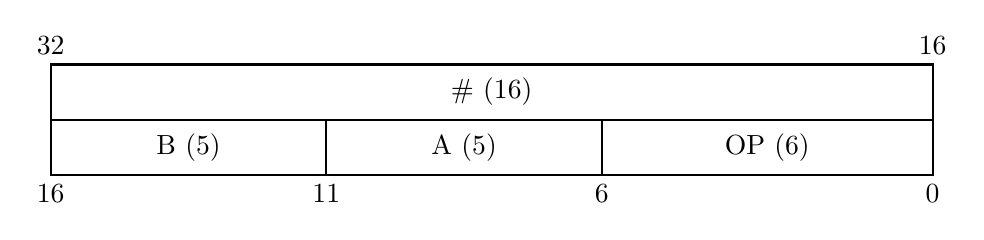
\begin{tikzpicture}[scale=.7]
\draw [thick] (0,0) rectangle (16,-1) node[pos=.5] {\# (16)};
\node[above] at (0, 0) {32};
\node[above] at (16, 0) {16};
\draw [thick] (0.0,-1) rectangle (5,-2) node[pos=.5] {B (5)};
\node[below] at (0, -2) {16};
\node[below] at (5, -2) {11};
\draw [thick] (5,-1) rectangle (10,-2) node[pos=.5] {A (5)};
\node[below] at (10, -2) {6};
\draw [thick] (10,-1) rectangle (16,-2) node[pos=.5] {OP (6)};
\node[below] at (16, -2) {0};
\end{tikzpicture}
\end{center}
\end{figure}

\chapter{Memory Management}
\label{ch:Memory Management}
\section{Segments}
\subsection{Base}
\subsection{Limit}
\section{Code Segment (CS)}
\section{Data Segment (DS)}
\section{Segment Switching}
\section{Changing Segments}

\chapter{Interrupts}
\label{ch:Interrupts}
\section{Interrupt Enabling/Disabling}
\label{sec:Interrupt Enabling/Disabling}
\subsection{Interrupt Enabled Flag}
\subsection{Internal Interrupt Mask}
\subsection{Programmable Interrupt Controller (PIC)}
\section{State Preservation}
\label{sec:State Preservation}
\subsection{Backup}
\subsection{Full Restore}
\subsection{Partial Restore}
\section{Interrupt Service Routine (ISR)}
\subsection{Interrupt Far Jump}
\subsection{Return to Context}
\subsection{Switch Context}

\chapter{I/O Conventions}
\label{ch:I/O Conventions}
\section{Reading Input}
\section{Writing Output}
\subsection{Problem with Interrupts}

\chapter{Instruction Set}
\label{ch:Instruction Set}
\clearpage

% MOVZ
\instruction{MOVZ / MOV=}{\underline{Mov}e if \underline{z}ero / \underline{Mov}e if equal}{
0x00: MOVZ a b \\
0x00: MOV= a b \emph{(Alternative notation)}
}{
Writes B to A if the zero flag is set. This instruction can also be used to only write B to A if, in the last comparison, B was equal to A. The alternative Memnonic MOV= was provided for this use. The comparison use of this instruction can only be expected to work if the last calculation was a compare or subtract instruction, and the used status flags haven't changed in the meanwhile.
}{
\begin{algorithmic}
\If {$Z$}
    \State $a\gets b$
\EndIf
\end{algorithmic}
alternative pseudocode:
\begin{algorithmic}
\If {$b_{previous} = a_{previous}$} \Comment Where $b_{previous}$ and $a_{previous}$ are the operands of a previous calculation
    \State $a\gets b$
\EndIf
\end{algorithmic}
}{}

% MOVNZ
\instruction{MOVNZ / MOV!=}{\underline{Mov}e if \underline{n}ot \underline{z}ero / \underline{Mov}e if not equal}{
0x01: MOVNZ a b \\
0x01: MOV!= a b \emph{(Alternative notation)}
}{
Writes B to A if the zero flag is clear. This instruction can also be used to only write B to A if, in the last comparison, B was unequal to A. The alternative Memnonic MOV= was provided for this use. The comparison use of this instruction can only be expected to work if the last calculation was a compare or subtract instruction, and the used status flags haven't changed in the meanwhile.
}{
\begin{algorithmic}
\If {$\neg Z$}
    \State $a\gets b$
\EndIf
\end{algorithmic}
alternative pseudocode:
\begin{algorithmic}
\If {$b_{previous} \not= a_{previous}$} \Comment Where $b_{previous}$ and $a_{previous}$ are the operands of a previous calculation
    \State $a\gets b$
\EndIf
\end{algorithmic}
}{}

% MOVS
\instruction{MOVS}{\underline{Mov}e if \underline{s}ign}{
0x02: MOVS a b
}{
Writes B to A if the sign flag is set.
}{
\begin{algorithmic}
\If {$S$}
    \State $a\gets b$
\EndIf
\end{algorithmic}
}{}

% MOVNS
\instruction{MOVNS}{\underline{Mov}e if \underline{n}ot \underline{s}ign}{
0x03: MOVNS a b
}{
Writes B to A if the sign flag is clear.
}{
\begin{algorithmic}
\If {$\neg S$}
    \State $a\gets b$
\EndIf
\end{algorithmic}
}{}

% MOVP
\instruction{MOVP}{\underline{Mov}e if \underline{p}arity}{
0x04: MOVP a b
}{
Writes B to A if the parity flag is set.
}{
\begin{algorithmic}
\If {$P$}
    \State $a\gets b$
\EndIf
\end{algorithmic}
}{}

% MOVNP
\instruction{MOVNP}{\underline{Mov}e if \underline{n}ot \underline{p}arity}{
0x05: MOVNP a b
}{
Writes B to A if the parity flag is clear.
}{
\begin{algorithmic}
\If {$\neg P$}
    \State $a\gets b$
\EndIf
\end{algorithmic}
}{}

% MOVO
\instruction{MOVO}{\underline{Mov}e if \underline{o}verflow}{
0x06: MOVO a b
}{
Writes B to A if the overflow flag is set.
}{
\begin{algorithmic}
\If {$O$}
    \State $a\gets b$
\EndIf
\end{algorithmic}
}{}

% MOVNO
\instruction{MOVNO}{\underline{Mov}e if \underline{n}o \underline{o}verflow}{
0x07: MOVNO a b
}{
Writes B to A if the overflow flag is clear.
}{
\begin{algorithmic}
\If {$\neg O$}
    \State $a\gets b$
\EndIf
\end{algorithmic}
}{}

% MOVC
\instruction{MOVC / MOVU>}{\underline{Mov}e if \underline{c}arry / \underline{Mov}e if \underline{u}nsigned greater}{
0x08: MOVC a b \\
0x08: MOVU> a b \emph{(Alternative notation)}
}{
Writes B to A if the carry flag is set. This instruction can also be used to only write B to A if, in the last comparison of unsigned numbers, B was greater than A. The alternative Memnonic MOVU> was provided for this use. The comparison use of this instruction can only be expected to work if the last calculation was a compare or subtract instruction, and the used status flags haven't changed in the meanwhile.
}{
\begin{algorithmic}
\If {$C$}
    \State $a\gets b$
\EndIf
\end{algorithmic}
alternative pseudocode:
\begin{algorithmic}
\If {$b_{previous} > a_{previous}$} \Comment Where $b_{previous}$ and $a_{previous}$ are the operands of a previous calculation
    \State $a\gets b$
\EndIf
\end{algorithmic}
}{}

% MOVNC
\instruction{MOVNC / MOVU<=}{\underline{Mov}e if \underline{n}o \underline{c}arry / \underline{Mov}e if \underline{u}nsigned smaller or equal}{
0x09: MOVNC a b \\
0x09: MOVU<= a b \emph{(Alternative notation)}
}{
Writes B to A if the carry flag is clear. This instruction can also be used to only write B to A if, in the last comparison of unsigned numbers, B was smaller than or equal to A. The alternative Memnonic MOVU<= was provided for this use. The comparison use of this instruction can only be expected to work if the last calculation was a compare or subtract instruction, and the used status flags haven't changed in the meanwhile.
}{
\begin{algorithmic}
\If {$\neg C$}
    \State $a\gets b$
\EndIf
\end{algorithmic}
alternative pseudocode:
\begin{algorithmic}
\If {$b_{previous} \leq a_{previous}$} \Comment Where $b_{previous}$ and $a_{previous}$ are the operands of a previous calculation
    \State $a\gets b$
\EndIf
\end{algorithmic}
}{}

% MOVU>=
\instruction{MOVU>=}{\underline{Mov}e if \underline{u}nsigned greater or equal}{
0x0A: MOVU>= a b
}{
Writes B to A if, in the last comparison of unsigned numbers, B was greater than or equal to A. The comparison use of this instruction can only be expected to work if the last calculation was a compare or subtract instruction, and the used status flags haven't changed in the meanwhile.
}{
\begin{algorithmic}
\If {$C \vee Z$}
    \State $a\gets b$
\EndIf
\end{algorithmic}
alternative pseudocode:
\begin{algorithmic}
\If {$b_{previous} \geq a_{previous}$} \Comment Where $b_{previous}$ and $a_{previous}$ are the operands of a previous calculation
    \State $a\gets b$
\EndIf
\end{algorithmic}
}{}

% MOVU<
\instruction{MOVU<}{\underline{Mov}e if \underline{u}nsigned smaller}{
0x0B: MOVU< a b
}{
Writes B to A if, in the last comparison of unsigned numbers, B was smaller than A. The comparison use of this instruction can only be expected to work if the last calculation was a compare or subtract instruction, and the used status flags haven't changed in the meanwhile.
}{
\begin{algorithmic}
\If {$\neg (C \vee Z)$}
    \State $a\gets b$
\EndIf
\end{algorithmic}
alternative pseudocode:
\begin{algorithmic}
\If {$b_{previous} < a_{previous}$} \Comment Where $b_{previous}$ and $a_{previous}$ are the operands of a previous calculation
    \State $a\gets b$
\EndIf
\end{algorithmic}
}{}



% MOVS>
\instruction{MOVS>}{\underline{Mov}e if \underline{s}igned greater}{
0x0C: MOVS> a b
}{
Writes B to A if, in the last comparison of signed numbers, B was greater than A. The comparison use of this instruction can only be expected to work if the last calculation was a compare or subtract instruction, and the used status flags haven't changed in the meanwhile.
}{
\begin{algorithmic}
\If {$\neg Z \wedge (O \oplus S)$}
    \State $a\gets b$
\EndIf
\end{algorithmic}
alternative pseudocode:
\begin{algorithmic}
\If {$b_{previous} > a_{previous}$} \Comment Where $b_{previous}$ and $a_{previous}$ are the operands of a previous calculation
    \State $a\gets b$
\EndIf
\end{algorithmic}
}{}

% MOVS<=
\instruction{MOVS<=}{\underline{Mov}e if \underline{s}igned smaller or equal}{
0x0D: MOVS<= a b
}{
Writes B to A if, in the last comparison of signed numbers, B was smaller than or equal to A. The comparison use of this instruction can only be expected to work if the last calculation was a compare or subtract instruction, and the used status flags haven't changed in the meanwhile.
}{
\begin{algorithmic}
\If {$Z \vee \neg(O \oplus S)$}
    \State $a\gets b$
\EndIf
\end{algorithmic}
alternative pseudocode:
\begin{algorithmic}
\If {$b_{previous} \leq a_{previous}$} \Comment Where $b_{previous}$ and $a_{previous}$ are the operands of a previous calculation
    \State $a\gets b$
\EndIf
\end{algorithmic}
}{}

% MOVS<
\instruction{MOVS<}{\underline{Mov}e if \underline{s}igned smaller}{
0x0E: MOVS< a b
}{
Writes B to A if, in the last comparison of signed numbers, B was smaller than A. The comparison use of this instruction can only be expected to work if the last calculation was a compare or subtract instruction, and the used status flags haven't changed in the meanwhile.
}{
\begin{algorithmic}
\If {$O \oplus S$}
    \State $a\gets b$
\EndIf
\end{algorithmic}
alternative pseudocode:
\begin{algorithmic}
\If {$b_{previous} < a_{previous}$} \Comment Where $b_{previous}$ and $a_{previous}$ are the operands of a previous calculation
    \State $a\gets b$
\EndIf
\end{algorithmic}
}{}

% MOVS>=
\instruction{MOVS>=}{\underline{Mov}e if \underline{s}igned greater or equal}{
0x0F: MOVS>= a b
}{
Writes B to A if, in the last comparison of signed numbers, B was greater than or equal to A. The comparison use of this instruction can only be expected to work if the last calculation was a compare or subtract instruction, and the used status flags haven't changed in the meanwhile.
}{
\begin{algorithmic}
\If {$\neg O \oplus S$}
    \State $a\gets b$
\EndIf
\end{algorithmic}
alternative pseudocode:
\begin{algorithmic}
\If {$b_{previous} \geq a_{previous}$} \Comment Where $b_{previous}$ and $a_{previous}$ are the operands of a previous calculation
    \State $a\gets b$
\EndIf
\end{algorithmic}
}{}

% MOV
\instruction{MOV}{\underline{Mov}e}{
0x10: MOV a b
}{
Writes B to A unconditionally.
}{
\begin{algorithmic}
\State $a\gets b$
\end{algorithmic}
}{}

% WRI
\instruction{WRI}{\underline{Wr}ite \underline{i}nterupts enabled}{
0x12: WRI \_ b
}{
Writes the least significant bit of B to the interrupts enabled flag. This allows you to enable and disable interrupts in a single instruction.
}{
\begin{algorithmic}
\State $I \gets b \mathrel{\&} 0001_{16}$ \Comment Everything but the least significant bit is omitted
\end{algorithmic}
}{I}

% ISTR
\instruction{ISTR}{\underline{I}nternal \underline{st}o\underline{r}e}{
0x14: ISTR a b
}{
Writes B to internal register A.
}{
\begin{algorithmic}
\State $a\gets b$ \Comment Where $a$ is an internal register
\end{algorithmic}
}{}

% ILD
\instruction{ILD}{\underline{I}nternal \underline{l}oa\underline{d}}{
0x15: ILD a b
}{
Writes internal register B to A.
}{
\begin{algorithmic}
\State $a\gets b$ \Comment Where $b$ is an internal register
\end{algorithmic}
}{}

% OUT
\instruction{OUT}{\underline{Out}put}{
0x16: OUT a b
}{
Writes B to output register A.
}{
\begin{algorithmic}
\State $a\gets b$ \Comment Where $a$ is an output register
\end{algorithmic}
}{}

% IN
\instruction{IN}{\underline{In}put}{
0x17: IN a b
}{
Request input from pheriperal B and write the returned input to A.
}{
\begin{algorithmic}
\State $a\gets \Call{RequestInputFrom}{b}$
\end{algorithmic}
}{}

% BACK
\instruction{BACK}{\underline{Back}up}{
0x18: BACK \_ \_
}{
Backups all the registers that have a backup registers
}{
\begin{algorithmic}
\State $bax \gets ax$
\State $bbx \gets bx$
\State $bcx \gets cx$
\State $bdx \gets dx$
\State $bex \gets ex$
\State $btm \gets tm$
\State $bsp \gets sp$
\State $bpc \gets pc$
\State $bsf \gets sf$ \Comment Backup the segment and flag registers
\end{algorithmic}
}{}

% FRET
\instruction{FRET}{\underline{F}ull \underline{re}s\underline{t}ore}{
0x19: FRET \_ \_
}{
Restores some of the registers and marks that the there is no interrupt being handled
}{
\begin{algorithmic}
\State $ax \gets bax$
\State $bx \gets bbx$
\State $cx \gets bcx$
\State $dx \gets bdx$
\State $ex \gets bex$
\State $tm \gets btm$
\State $sp \gets bsp$
\State $pc \gets bpc$
\State $sf \gets bsf$ \Comment Restore the segment and flag registers
\State \Call{MarkInterruptEnded}{ } \Comment Unlock the internal lock that prevents interrupts
\end{algorithmic}
}{Z, S, P, O, C and I}

% PRET
\instruction{PRET}{\underline{P}artial \underline{re}s\underline{t}ore}{
0x1A: PRET \_ \_
}{
Restores some of the registers and marks that the there is no interrupt being handled.
}{
\begin{algorithmic}
\State $pc \gets bpc$
\State $sf \gets bsf$ \Comment Restore the segment and flag registers
\State \Call{MarkInterruptEnded}{ } \Comment Unlock the internal lock that prevents interrupts
\end{algorithmic}
}{Z, S, P, O, C and I}

% FJMP
\instruction{FJMP}{\underline{F}ar \underline{j}u\underline{mp}}{
0x1B: FJMP \_ \_
}{
Restores some of the registers.
}{
\begin{algorithmic}
\State $pc \gets bpc$
\State $sf \gets bsf$ \Comment Restore the segment and flag registers
\end{algorithmic}
}{Z, S, P, O, C and I}

% HLT
\instruction{HLT}{\underline{H}a\underline{lt}}{
0x1C: HLT \_ \_
}{
Halts the CPU until an external interrupt is triggered and resumes.
}{
\begin{algorithmic}
\State \Call{HaltCPU}{ }
\end{algorithmic}
}{}

% NOP
\instruction{NOP}{\underline{N}o \underline{op}erations}{
0x1D: NOP \_ \_
}{
Does nothing but delay the cpu a minimal amount of cycles. 
}{
\begin{algorithmic}
\If {$false$} \Comment NOP is implemented as a do never conditional
    \State $...$ 
\EndIf
\end{algorithmic}
}{}

% OR
\instruction{OR}{Bitwise \underline{or}}{
0x20: OR a b \\
0x21: OR !a b \\
0x22: OR a !b \\
0x23: OR !a !b \\
0x23: NAND a b \emph{(Alternative notation)}
}{
preforms bitwise logical or operation on A and B and writes the answer to A. The answer is also evaluated to update the status flags. Both operands can be One's Complement Negated (NOT'ed) before the operation in the same instruction. This is marked by the '!' before the operand. 
}{
\begin{algorithmic}
\State $y\gets (!)a \mathrel{|} (!)b$
\State $a\gets y$
\State $Z, S, P\gets \Call{EvaluateAnswer}{y}$
\end{algorithmic}
}{Z, S and P}

% AND
\instruction{AND}{Bitwise \underline{and}}{
0x24: AND a b \\
0x25: AND !a b \\
0x26: AND a !b \\
0x27: AND !a !b \\
0x27: NOR a b \emph{(Alternative notation)}
}{
preforms bitwise logical and operation on A and B and writes the answer to A. The answer is also evaluated to update the status flags. Both operands can be One's Complement Negated (NOT'ed) before the operation in the same instruction. This is marked by the '!' before the operand. 
}{
\begin{algorithmic}
\State $y\gets (!)a \mathrel{\&} (!)b$
\State $a\gets y$
\State $Z, S, P\gets \Call{EvaluateAnswer}{y}$
\end{algorithmic}
}{Z, S and P}

% XOR
\instruction{XOR}{Bitwise e\underline{x}clusive \underline{or}}{
0x28: XOR a b \\
0x29: XOR !a b \\
0x29: XAND a b \emph{(Alternative notation)} \\
0x2A: XOR a !b \emph{(Artifact instruction)}\\
0x2B: XOR !a !b \emph{(Artifact instruction)}
}{
preforms bitwise logical exclusive or operation on A and B and writes the answer to A. The answer is also evaluated to update the status flags. Both operands can be One's Complement Negated (NOT'ed) before the operation in the same instruction. This is marked by the '!' before the operand. However because of the logical properties of exclusive or, "XOR !a !b" and "XOR a !b" behave exactly the same as "XOR a b" and "XOR !a b" respectively. Thus instruction "XOR !a !b" and "XOR a !b" are deemed to be artifact instructions and shouldn't be used.
}{
\begin{algorithmic}
\State $y\gets (!)a \mathrel{^\wedge} (!)b$
\State $a\gets y$
\State $Z, S, P\gets \Call{EvaluateAnswer}{y}$
\end{algorithmic}
}{Z, S and P}

% ADD
\instruction{ADD / SUB}{\underline{Add}ition / \underline{Sub}traction}{
0x28: ADD a b \\
0x29: ADD -a b \\
0x2A: ADD a -b \\
0x2A: SUB a b \emph{(Alternative notation)}
}{
adds A to B and writes the answer to A. The addition is checked on overflow and carry and the answer is also evaluated to update the status flags. Both operands can be Two's Complement Negated before the operation in the same instruction. This is marked by the '-' before the operand.
}{
\begin{algorithmic}
\State $y\gets (-)a + (-)b$
\State $a\gets y$
\State $O, C\gets \Call{CheckAddition}{ }$
\State $Z, S, P\gets \Call{EvaluateAnswer}{y}$
\end{algorithmic}
}{Z, S, P, O and C}

% ADD1
\instruction{ADD1 / SUB1}{\underline{Add}ition plus \underline{1} / \underline{Sub}traction minus \underline{1}}{
0x28: ADD1 a b \emph{(Artifact instruction)}\\
0x29: ADD1 -a b \emph{(Artifact instruction)}\\
0x2A: ADD1 a -b \emph{(Artifact instruction)}\\
0x2A: SUB1 a b \emph{(Artifact instruction)} \emph{(Alternative notation)}
}{
adds A and 1 to B and writes the answer to A. The addition is checked on overflow and carry and the answer is also evaluated to update the status flags. Both operands can be Two's Complement Negated before the operation in the same instruction. This is marked by the '-' before the operand. If one of the operands is negated the extra 1 will be negated as well
}{
\begin{algorithmic}
\State $y\gets (-)a + (-)b + (-)1$
\State $a\gets y$
\State $O, C\gets \Call{CheckAddition}{ }$
\State $Z, S, P\gets \Call{EvaluateAnswer}{y}$
\end{algorithmic}
}{Z, S, P, O and C}

% ADDC
\instruction{ADDC / SUBB}{\underline{Add}ition with \underline{c}arry / \underline{Sub}traction with \underline{b}orrow}{
0x28: ADDC a b \\
0x29: ADDC -a b \\
0x2A: ADDC a -b \\
0x2A: SUBB a b \emph{(Alternative notation)}
}{
adds A to B and writes the answer to A, however, if the carry flag is set an extra 1 will be added to the sum. The addition is checked on overflow and carry and the answer is also evaluated to update the status flags. Both operands can be Two's Complement Negated before the operation in the same instruction. This is marked by the '-' before the operand. If one of the operands is negated the extra 1 will be negated as well.
}{
\begin{algorithmic}
\State $y\gets (-)a + (-)b + (-)C$
\State $a\gets y$
\State $O, C\gets \Call{CheckAddition}{ }$
\State $Z, S, P\gets \Call{EvaluateAnswer}{y}$
\end{algorithmic}
}{Z, S, P, O and C}

% 
\instruction{}{\underline{}}{
0x:  a b
}{

}{
\begin{algorithmic}
\State $a\gets b$
\end{algorithmic}
}{}


% Appendix
\appendix
%\backmatter
\chapter{Instruction Set Listings}
\label{app:Instruction Set Listings}
\begin{center}
\begin{longtable}{ccclcc}
\hiderowcolors
\caption{List of instructions sorted by opcode} 
\label{tab:opcode_sorted_instructions_list} \\
\multicolumn{3}{c}{\textbf{Opcode}} & \multirow{2}{*}{\textbf{Memnonic}} & \multirow{2}{*}{\textbf{Operand A}} & \multirow{2}{*}{\textbf{Operand B}} \\
\textbf{Decimal} & \textbf{Hex} & \textbf{Binary} &  &  &  \\ \hline 
\showrowcolors 
\endhead
0  & 0x00 & 000000 & MOVZ  \& MOV=   & W?    & R?  \\
1  & 0x01 & 000001 & MOVNZ \& MOV!=  & W?    & R?  \\
2  & 0x02 & 000010 & MOVS            & W?    & R?  \\
3  & 0x03 & 000011 & MOVNS           & W?    & R?  \\
4  & 0x04 & 000100 & MOVP            & W?    & R?  \\
5  & 0x05 & 000101 & MOVNP           & W?    & R?  \\
6  & 0x06 & 000110 & MOVO            & W?    & R?  \\
7  & 0x07 & 000111 & MOVNO           & W?    & R?  \\
8  & 0x08 & 001000 & MOVC  \& MOVU>  & W?    & R?  \\
9  & 0x09 & 001001 & MOVNC \& MOVU<= & W?    & R?  \\
10 & 0x0A & 001010 & MOVU>=          & W?    & R?  \\
11 & 0x0B & 001011 & MOVU<           & W?    & R?  \\
12 & 0x0C & 001100 & MOVS>           & W?    & R?  \\
13 & 0x0D & 001101 & MOVS<=          & W?    & R?  \\
14 & 0x0E & 001110 & MOVS<           & W?    & R?  \\
15 & 0x0F & 001111 & MOVS>=          & W?    & R?  \\
16 & 0x10 & 010000 & MOV             & W     & R   \\
17 & 0x11 & 010001 & n/a             & n/a   & n/a \\
18 & 0x12 & 010010 & WRI             & \_    & R   \\
19 & 0x13 & 010011 & n/a             & n/a   & n/a \\
20 & 0x14 & 010100 & STRB            & O     & R   \\
21 & 0x15 & 010101 & LDB             & W     & O   \\
22 & 0x16 & 010110 & OUT             & O     & R   \\
23 & 0x17 & 010111 & IN              & W     & O   \\
24 & 0x18 & 011000 & BACK            & \_    & \_  \\
25 & 0x19 & 011001 & FRET            & \_    & \_  \\
26 & 0x1A & 011010 & PRET            & \_    & \_  \\
27 & 0x1B & 011011 & FJMP            & \_    & \_  \\
28 & 0x1C & 011100 & HLT             & \_    & \_  \\
29 & 0x1D & 011101 & NOP             & \_    & \_  \\
30 & 0x1E & 011110 & CMP             & R     & R   \\
31 & 0x1F & 011111 & TEST            & R     & R   \\
32 & 0x20 & 100000 & OR              & R\&W  & R   \\
33 & 0x21 & 100001 & OR              & !R\&W & R   \\
34 & 0x22 & 100010 & OR              & R\&W  & !R  \\
35 & 0x23 & 100011 & OR              & !R\&W & !R  \\
36 & 0x24 & 100100 & AND             & R\&W  & R   \\
37 & 0x25 & 100101 & AND             & !R\&W & R   \\
38 & 0x26 & 100110 & AND             & R\&W  & !R  \\
39 & 0x27 & 100111 & AND             & !R\&W & !R  \\
40 & 0x28 & 101000 & XOR             & R\&W  & R   \\
41 & 0x29 & 101001 & XOR             & !R\&W & R   \\
42 & 0x2A & 101010 & XOR             & R\&W  & !R  \\
43 & 0x2B & 101011 & XOR             & !R\&W & !R  \\
44 & 0x2C & 101100 & ADD             & R\&W  & R   \\
45 & 0x2D & 101101 & ADD             & !R\&W & R   \\
46 & 0x2E & 101110 & ADD   \& SUB    & R\&W  & !R  \\
47 & 0x2F & 101111 & n/a             & n/a   & n/a \\
48 & 0x30 & 110000 & ADD1            & R\&W  & R   \\
49 & 0x31 & 110001 & ADD1            & !R\&W & R   \\
50 & 0x32 & 110010 & ADD1  \& SUB1   & R\&W  & !R  \\
51 & 0x33 & 110011 & n/a             & n/a   & n/a \\
52 & 0x34 & 110100 & ADDC            & R\&W  & R   \\
53 & 0x35 & 110101 & ADDC            & !R\&W & R   \\
54 & 0x36 & 110110 & ADDC  \& SUBB   & R\&W  & !R  \\
55 & 0x37 & 110111 & n/a             & n/a   & n/a \\
56 & 0x38 & 111000 & SHL             & W     & R   \\
57 & 0x39 & 111001 & SHL1            & W     & R   \\
58 & 0x3A & 111010 & RCL             & W     & R   \\
59 & 0x3B & 111011 & ROL             & W     & R   \\
60 & 0x3C & 111100 & SHR             & W     & R   \\
61 & 0x3D & 111101 & SHR1            & W     & R   \\
62 & 0x3E & 111110 & RCR             & W     & R   \\
63 & 0x3F & 111111 & ROR             & W     & R   \\
\end{longtable}
\end{center}

\chapter{Simplified Mnemonics}

\chapter{Common Procedures}

\chapter{Standard Peripherals}
\section{Programmable Interrupt Controller (PIC)}
\section{Keyboard}
\section{Programmable Interrupt Timer (PIT)}
\section{Sound Card}
\section{Graphical Card}
\section{Memory Control Hub (MCH)}
\section{Segements and Out Of Bounds Exception}

\end{document}

